\section{Definicions}
Abans de parlar sobre els tipus de llicencies software s'haurien 
de conèixer alguns conceptes bàsics.

\begin {itemize}
	\item \emph{Llicencies de software}: són un contracte entre el desenvolupador 
	del software (sotmès a propietat intel·lectual i els drets d'autor), i l'usuari. 
	En aquest contracte es defineixen els drets i deures de ambdues parts. El 
	desenvolupador, o qui hagi cedit els drets d'explotació del producte, és 
	la persona que decideix quina llicencia software usar per la distribució del 
	programa.
	\item \emph{Patent}: és el conjunt de drets exclusius concedits per un estat al 
	creador o als creadors de un producte susceptible a ser explotat industrialment, 
	per un període limitat de temps a canvi de la divulgació de la invenció. Implica,
	bàsicament, que tercers no poden fer ús de la tecnologia patentada. \cite {definicions}
	\item \emph{Drets d'autor o \textit{copyright}}: és un conjunt de drets i normes \cite {copyright}
	que tenen els autors de creacions de obres de qualsevol tipus, tant científica, 
	tecnològica, didàctica, etc.
\end {itemize}

\section{Tipus de llicencies software}
Hi han molts tipus de llicencies software, però les més utilitzades són aquestes quatre:

\begin{itemize}
	\item \emph{GPL}: prové de \emph{GNU Public License} (GNU essent acrònim de
	\emph{GNU no és Unix}). Aquesta 
	llicència permet la copia, la distribució, tant amb finalitats comercial com no, i 
	la modificació del codi només si es segueix utilitzant el mateix 
	tipus de llicencia, la GPL. No permet la distribució d'executables sense mostrar 
	el codi font d'aquest. És la més usada en el món del 
	software lliure, i garanteix a l'usuari final la llibertat de usar, estudiar, compartir 
	i modificar el software amb el propòsit d'evitar que el software tingui una 
	llicencia de software privativa i protegir-lo dels intents d'apropiació que 
	restringeixin les llibertats de l'usuari.
	
	Si tú utilitzes llibreries amb codi llicenciat GPL, o les modifiques, també has de compartir el teu codi i/o modificacions amb la llicència GPL.
	
	Aquesta llicencia va ser creada per
	\emph{Richard Stallman}, fundador de la \emph{Free Software Foundation}
	pel projecte del grup \emph{GNU}.
	Segons aquest grup, quan es parla de que és \textit{free} es refereixen a que és 
	lliure, no gratuït. \cite {gnugpl} \cite {tldr}
	\item \emph{BSD}: o \emph{Berkeley Software Distribution} és una llicencia software més 
	permissiva que GPL, ja que aquesta té menys restriccions en comparació a la 
	anterior. La llicència BSD, al contrari 
	que la GPL permet l'ús del codi font en software no lliure. Es podria definir com a \emph{llicència molt liberal}. Molts sistemes operatius descendents de BSD són \emph{SunOS, 
	FreeBSD i MacOS X}, entre altres. \cite {bsd} \cite {tldr}
	\item \emph{MIT}: La llicència MIT (Massachusetts Institute of Technology)
	té unes característiques molt similars a la llicència BSD:
	pots fer el que vulguis amb el teu software mentre tu adjuntis el copyright 
	inicial. Hi ha molt software que utilitza la llicència MIT, ja que és simple d'entendre i curta; projecte \emph{Mono}, o \emph{Ruby on Rails}, entre moltes altres.\cite {mit} \cite {tldr}
	\item \emph{WTFPL}: és la llicència més permissiva. Bàsicament, et permet fer
	el que vulguis amb el teu programa com el mateix nom de la llicència indica:
	\emph{Do What The Fuck You Want To The Public Licence}.
	L'usuari pot fer el que vulgui amb el codi font i la llicència en sí, sense
	cap mena de restricció. Aquesta llicència és poc utilitzada, degut a la seva
	falta de restriccions, i el fet que no assegura la continuïtat de les llibertats
	que ella mateixa proporciona.\cite {tldr}
	\item \emph{MPL}: la \emph{Mozilla Public License} és una llicència no lucrativa i poc estricta, que només té uns requeriments molt senzills.
	Els programes que utilitzen aquesta llicència són bàsicament els de la \emph{Mozilla Foundation},
	per exemple el navegador \emph{Firefox} o el client de correus \emph{Thunderbird},
	però també és usat per altres programes, com per la companyia \emph{Adobe} en
	la seva línia de productes \emph{Flex}, o per \emph{LibreOffice}, popular suite
	d'ofimàtica. \cite {tldr}
	
	\item \emph{Sense llicència}: quan un programa no especifica una llicència, l'usuari només té dret a \emph{observar} el codi font d'aquest. Es reserven tots els drets a l'autor, que pot fer el que vulgui amb el programa.
\end{itemize}

\begin{figure}[ht!]
\centering
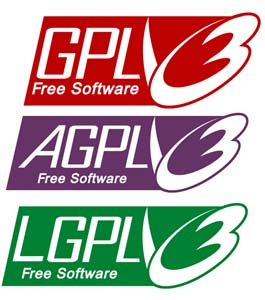
\includegraphics[width=45mm]{data/gpls.jpg}
\caption{Logotips de les diferents versions de la llicència \emph{GNU GPL}.}
\label{gpls}
\end{figure}

\section{Decidir la llicència}
Quan el desenvolupador (o companyia) ha de decidir quin tipus de llicència vol
usar per el seu software ha de tenir en compte les seves motivacions: si aquest
vol remuneració monetària, usarà una llicència de software privativa, la qual estipularà que el seu producte no pot ser compartit ni modificat, o si vol que el seu producte estigui l'abast de 
la comunitat, en aquest cas haurà de decidir el grau de llibertat que vol que tingui 
l'usuari.

De totes formes, cal mencionar la possibilitat de obtenir remuneració econòmica amb llicències
de software lliures: ja sigui a partir de donacions (el mètode més habitual), o amb la
venda directa de l'executable.
